\ylDisplay{Kast kaubikus} % Ülesande nimi
{Oleg Košik} % Autor
{lõppvoor} % Voor
{2009} % Aasta
{G 2} % Ülesande nr.
{3} % Raskustase
{
% Teema: Staatika
\ifStatement
Kast massiga $m=\SI{15}{kg}$ on kinnitatud kaubiku tagaseina külge nööriga. Leida nööri pinge minimaalne võimalik väärtus äkkpidurduse ajal, kui kiirusega $v_0=\SI{45}{km/h}$ sõitev kaubik jääb seisma ajaga $t=\SI{5}{s}$. Hõõrdetegur kasti aluse ja kaubiku põranda vahel $\mu=\num{0,2}$, nurk nööri ja kaubiku tagaseina vahel $\alpha=\SI{45}{\degree}$. Lugeda, et pidurdamine oli ühtlane ja kast püsis kogu aeg paigal.
\begin{center}
	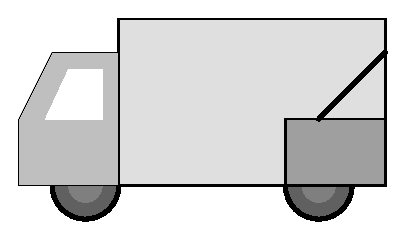
\includegraphics[width=0.5\linewidth]{2009-v3g-02-G_kast_kaubikus.eps}
\end{center}
\fi


\ifHint
Koheldes hõõrdejõudu tundmatuna, võime kasti jaoks kirja panna Newtoni II seaduse nii $x$- kui ka $y$-telje jaoks. Hõõrdejõu maksimaalne väärtus on $F_\mu = N\mu$, kus $N$ on toereaktsioon.
\fi


\ifSolution
Kaubiku kiirendus on $a=v_0/t=\SI{2.5}{m/s^2}$. Newtoni II seaduse põhjal
\[
\vec{N}+\vec{T}+\vec{F_h}+m\vec{g}=m\vec{a}.
\]
Nööri pinge on minimaalne, kui hõõrdejud $F_h$ saavutab maksimaalse väärtuse $\mu N$. Projektsioon $x$-teljele:
\[
T\sin\alpha+\mu N=ma;
\]
$y$-teljele:
\[
N+T\cos\alpha-mg=0.
\]
Lahendades süsteemi leiame, et
\[
T=m\frac{a-\mu g}{\sin\alpha-\mu\cos\alpha} \approx \SI{14}{N}.
\]
\fi
}